\titre{Exercice 1 :}
\begin{enumerate}
	\item 
		\begin{enumerate}
			\item
				\begin{itemize}
					\item $E ::= T_X T_Y $
					\item $X ::= a$
					\item $T_X ::= X | XT_X$
					\item $Y ::= a | b | c$
					\item $T_Y ::= \varepsilon | YT_Y$
				\end{itemize}
			\item
				\begin{itemize}
					\item $E ::= T_YT_x$
					\item $T_Y ::= \varepsilon | aT_Y | bT_Y | cT_Y$
					\item $T_X ::= a | aT_X$
				\end{itemize}
			\item
				\begin{itemize}
					\item $E ::= XY$
					\item $X ::= \varepsilon | aX | bX$
					\item $Y ::= \varepsilon | bX | cX$
				\end{itemize}
			\item
				\begin{itemize}
					\item $E ::= YaaZ$
					\item $Z ::= \varepsilon | abZ | bcZ | caZ$
					\item $Y ::= \varepsilon | abY | bCY$
					\item $C ::= \varepsilon | cC$
				\end{itemize}
			\item 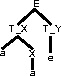
\includegraphics[width=60px]{Images/fig4.pdf} 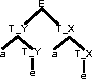
\includegraphics[width=100px]{Images/fig5.pdf} 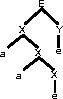
\includegraphics[width=50px]{Images/fig6.pdf}
		\end{enumerate}
	\item
		\begin{enumerate}
			\item $E ::= \varepsilon | aEb$
			\item $E ::= \varepsilon | c | d | e | cEc | dEd | eEe$
			\item $E ::= \varepsilon | (E)E$
			\item 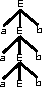
\includegraphics[width=30px]{Images/fig7.pdf} 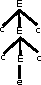
\includegraphics[width=30px]{Images/fig8.pdf} 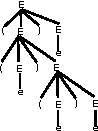
\includegraphics[width=50px]{Images/fig9.pdf}
		\end{enumerate}
	\item 
		\begin{enumerate}
			\item 
				\begin{itemize}
					\item $E ::= XY$
					\item $X ::= \varepsilon | aXb$
					\item $Y ::= \varepsilon | cYd$
				\end{itemize}
			\item
				\begin{itemize}
					\item $E ::= X | aEd$
					\item $X ::= \varepsilon | bXc$
				\end{itemize}
			\item
				\begin{itemize}
					\item $G ::= E | F$
					\item $E ::= XY$
					\item $X ::= \varepsilon | aXb$
					\item $Y ::= \varepsilon | cYd$
					\item $F ::= Z | aFd$
					\item $Z ::= \varepsilon | bZc$
				\end{itemize}
			\item 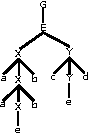
\includegraphics[width=50px]{Images/fig10.pdf} 
\includegraphics[width=30px]{Images/fig11.pdf} 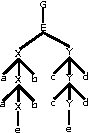
\includegraphics[width=50px]{Images/fig12.pdf}
		\end{enumerate}

	\item 
		\begin{enumerate}
			\item 
				\begin{itemize}
					\item $E ::= \varepsilon | ZE$
					\item $Z ::= aEbb | bEaEb | bbEa$
				\end{itemize}
			\item 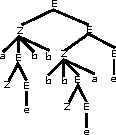
\includegraphics[width=70px]{Images/fig13.pdf} 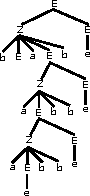
\includegraphics[width=50px]{Images/fig14.pdf}
			\item C'est l'ensemble des mots qui ont deux fois plus de $b$ que de $a$
		\end{enumerate}

	\item 
		\begin{enumerate}
			\item $E ::= \varepsilon | aEbE | bEaE$
			\item $E = (1 + aEb + bEa)*$
			\item 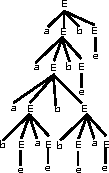
\includegraphics[width=70px]{Images/fig15.pdf}
		\end{enumerate}
\end{enumerate}

\titre{Exercice 2}
\begin{enumerate}
	\item 
		\begin{enumerate}
		\item 
			\begin{itemize}
				\item $E ::= [L]$ : un crochet, puis une liste, puis un crochet
				\item $L ::= \varepsilon | PU$ : rien ou (un nombre du langage, puis une liste éventuellement vide commençant par une virgule)
				\item $U ::= \varepsilon | ,PU$ : une partie de la liste ',' puis un nombre du langage puis une liste $\rightarrow$ liste commençant par une virgule
				\item $P ::= 0Z | SN$ : un nombre du langage (que des zéros ou un signe et un nombre ne commençant pas par 0)
				\item $Z ::= \varepsilon | 0Z$ : des 0 les uns à côté des autres
				\item $N ::= 1M | 2M | 3M | 4M | 5M | 6M | 7M | 8M | 9M $ : commence par autre chose que 0 puis des chiffres entre O et 9
				\item $M ::= \varepsilon | 0M | N$ : des chiffres entre 0 et 9 qui se suivent
				\item $S ::= \varepsilon | + | -$ : le signe
			\end{itemize}
		\item 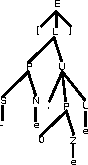
\includegraphics[width=70px]{Images/fig16.pdf}
		\end{enumerate}

	\item 
		\begin{itemize}
			\item $N = (\varepsilon + '+' + '-') (0^* + (1+2+3+4+5+6+7+8+9)(0+1+2+3+4+5+6+7+8+9)^*)$
			\item $R = [] + [N(,N)^*]$
			\item Oui ce langage est régulier
		\end{itemize}

	\item 
		\begin{enumerate}
			\item $E ::= \varepsilon | 0 | 1 | a | b | c | d | E+E | EE | E* | (E)$
			\item Elle est ambigue (exemple : $aaa$)
			\item 
		\end{enumerate}
\end{enumerate}
